\clearpage
\subsection{Procedure Declarations} % (fold)
\label{sub:proc_decl-procedure_declarations}

Procedures contain code that define the steps the computer performs when the procedure is called. In your Program you can define your own Procedures, allowing you to divide a program's tasks into separate Procedures.

\begin{figure}[h]
   \centering
   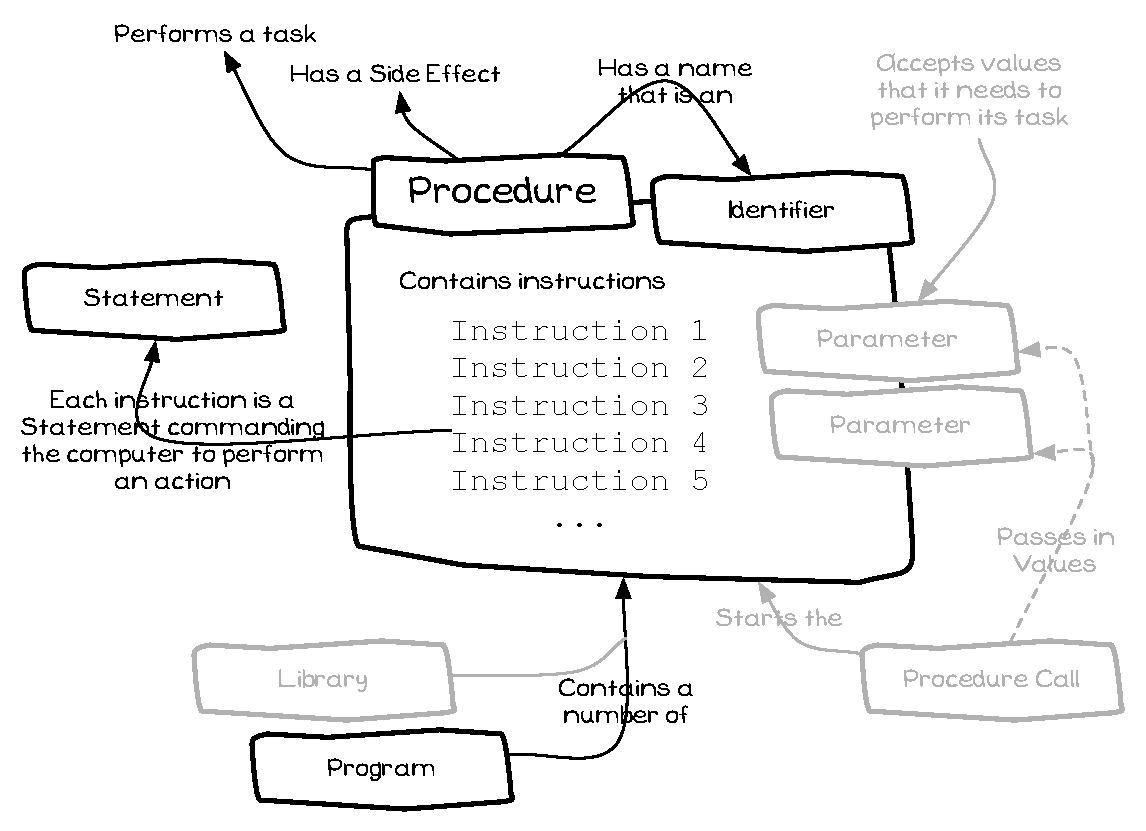
\includegraphics[width=\textwidth]{./topics/program-creation/diagrams/ProcedureDeclaration} 
   \caption{Procedure Declaration}
   \label{fig:procedure-decl-procedure-decl}
\end{figure}

\mynote{
\begin{itemize}
  \item A Procedure is an \textbf{artefact} that you can \emph{create} and \emph{use} in your code.
  \item Each Procedure contains code to perform a certain task. When you want the task performed you call the Procedure.
  \item Procedures should have a \textbf{side effect}\footnote{Output to the Terminal is an example of a Side Effect. After calling these procedures the text you wanted to appear was written to the Terminal. These Procedures changed the Terminal.}, meaning that it changes something when it is executed.
  \item The Procedure's declaration defines its \textbf{name}, and the \textbf{steps} it performs.
  \item Each instructions in the Procedure is a \nameref{sub:statement}.
  \item The Procedure's \nameref{sub:identifier}:
  \begin{itemize}
    \item Is the name used to call the Procedure.
    \item Should be a \textbf{verb} that \textbf{reflects the task} the Procedure performs.
  \end{itemize} 
  \item When the Procedure is called its instructions are executed.
  \item Each Procedure's instructions are isolated from the other code in your Program. When you are working on a Procedure you do not need to know about the internal workings of the other procedures.
\end{itemize}
}

% subsection procedure_declarations (end)